\chapter{Data Mining}
\label{chap:dataMining}
Virtual Observatory may be seen as data infrastructure. It enables
astronomers to get data more easily in a uniform way. But there is
another and even bigger problem now. How to deal with such amount of
data? Can we change the problem to opportunity? Can we discover new
phenomena, new types of objects or exploit natural groups in the data?
Data Mining and related techniques are created exactly for such
purposes. Used correctly, it can be powerful approach, promising
scientific advance. On the other side this field is very complex with
dozens of different methods and algorithms. This forms needs and
opportunity for interdisciplinary cooperation with Data Mining
experts. This can be very beneficially for both fields, providing
astronomers with interesting methods for data analysis and computer
scientist with large ammout of quality data.

\section{Supervised Methods}
These methods are also known as predictive\cite{ball2010data}. They
rely on training set with known target property. This set must be
representative. The selected method is trained on that set and the
result is then used on data for which the target property is not
known. Among supervised method are classification, regression, anomaly
detection and others.

\subsection{Decision Tree (DT)}
Is an example of supervised classification. Based on final number of
data $(x^{(1)},\ldots,x^{(p)})$ with known class $C_1,\ldots, C_m$
classifier is created, i.e. image $f$ classifying any $x \in
\mathcal{X}, f:\mathcal{X}\rightarrow \mathcal{Y}$, where
$\mathcal{X}$ is a set of possible input vectors and $\mathcal{Y}$ is
a set which values represents classes $C_1,\ldots, C_m$ (for example
$\mathcal{Y} = {1,\ldots,m}$). The model is consctructed based on
traning set as a tree structure, where leaves represent
classifications and branches conjunctions of features that lead to
those classifications. The main advatages of DT are:

\begin{itemize}
\item Simple to understand and interpret.
\item Able to handle both numerical and categorical data.
\item Uses a white box model.
\item Perform well with large data in a short time.
\end{itemize}

In pseudocode, the general algorithm for building decision trees is
\cite{kotsiantis2007supervised}:
\begin{enumerate}
\item Check for base cases
\item For each attribute a
  \begin{itemize}
  \item Find the normalized information gain from splitting on a
  \end{itemize}
\item Let "a best" be the attribute with the highest normalized information gain
\item Create a decision node that splits on "a best"
\item Recur on the sublists obtained by splitting on "a best", and add
  those nodes as children of node
\end{enumerate}

Furtheremore algoritms C4.5 is described for several reasons: Its code
is aviable and free implementeations exist (J48 in weka), is de-facto
standard in classsifiction using DT, is used in practical part of this
work. The key question of DT algoritm is how to choose attribute for
splitting the tree. C4.5 Uses meassures based on information entropy:

\begin{equation}
  \label{eq:entropy}
  H(X) = -\sum_{i=1}^n {p(x_i) \log_2 p(x_i)},
\end{equation}
where $p(x_i)$ is probability of occurrence of class $i$ and $n$ is the
number of classes.

After the tree is created it is optimized by pruning, which prevent
over-fitting.

%\subsubsection{Pruning}         
\subsubsection{Cross-validation}
The quality of the training set is crucial to good results. The amount
of data for testing is always limited. In general, one cannot be sure
whether a sample is representative. If for example certain group is
missing, one could not expect a classifier learned from such data to
perform well on the examples s of that class. One of the technique used
here is cross-validation.

The data is divided into fixed number of partitions and each in turn
is used for testing and the reminder is used for training. Finally,
the number of partitions error estimates are averaged to yield an
overall error. The standard is to used 10-fold cross-validation. This
number is a result of tests on numerous data sets \cite{witten2005data}

\subsubsection{Example: Classifying Galaxies Stars and QSO}
There is an example of classifying Galaxies Stars and QSO based on
photometric properties using Decision Tree algorithm J48 (C4.5 in
Weka). The data are from SDSS (Sloan Digital Sky Survey) DR7. 298
Objects were used (100 Stars, 99 Galaxies, 99 QSO). SDSS Filters
u,g,r,i were used as parameters. Data were obtained using SQL query
from SDSS CAS.

\begin{lstlisting}
SELECT TOP 100 u-g,g-r,r-i,s.specClass
FROM PhotoPrimary p join SpecPhotoAll s on p.objid=s.objid 
WHERE s.specClass in (1)
AND u between 18 and 19
UNION all
SELECT top 100 u-g,g-r,r-i,s.specClass
FROM PhotoPrimary p join SpecPhotoAll s on p.objid=s.objid 
WHERE s.specClass in (2)
AND u between 18 and 19
UNION all
SELECT top 100 u-g,g-r,r-i,s.specClass
FROM PhotoPrimary p join SpecPhotoAll s on p.objid=s.objid 
WHERE s.specClass in (3)
AND u between 18 and 19
\end{lstlisting}

The following listing shows the result of classification. The
classifier was able to distinguish 95\% of the processed objects.

\begin{table}[ht]
  \centering
  \small
     \begin{tabular}[ht]{l r@{,}l r@{,}l l l}
     \toprule
     Filter & Wavelength [$\AA$] \\
     \midrule
     Ultraviolet (u) & 3543 \\
     Green (g) & 4770\\
     Red (r) & 6231\\
     Near Infrared (i) & 7625\\
     Infrared (z) & 9134 \\
     \bottomrule
   \end{tabular}
  \caption{SDSS Filters}
  \label{tab:SDSSFilter}
\end{table}


\begin{lstlisting}
Correctly Classified Instances          96               95.0495 %
Incorrectly Classified Instances         5                4.9505 %
Kappa statistic                          0.9257
Mean absolute error                      0.0669
Root mean squared error                  0.1778
Relative absolute error                 15.0587 %
Root relative squared error             37.6973 %
Total Number of Instances              101     
\end{lstlisting}

The big advantage of Decision Trees over black box algorithms (such as
Neural Network) is that one could understand the classification
process. The decision tree generated for this example is following:

\begin{lstlisting}
  ug <= 0.663668
|   gr <= -0.191208: 1 (7.0)
|   gr > -0.191208: 3 (104.0/5.0)
ug > 0.663668
|   ri <= 0.285854: 1 (88.0/5.0)
|   ri > 0.285854
|   |   ri <= 0.314657
|   |   |   gr <= 0.692108: 2 (6.0)
|   |   |   gr > 0.692108: 1 (3.0)
|   |   ri > 0.314657: 2 (90.0/2.0)
\end{lstlisting}

Useful tool for understanding how classifier was successful on
individual classes is the confusion matrix. Columns shows how the
object was classified and the row what is his actual class. In this
example QSO were classified correctly in 100\% cases. Distinction
between stars and galaxies are a bit worse and the algorithm classify 2
galaxies incorrectly as stars and two stars were confused with
galaxies. On stars was incorrectly classified as QSO.
 
\begin{lstlisting}
  s  g  q   <-- classified as
 30  2  1 |  s 
  2 33  0 |  g 
  0  0 33 |  q 
\end{lstlisting}

\begin{figure}[!htbp]
%      \begin{center}
        \leavevmode
        \ifpdf
        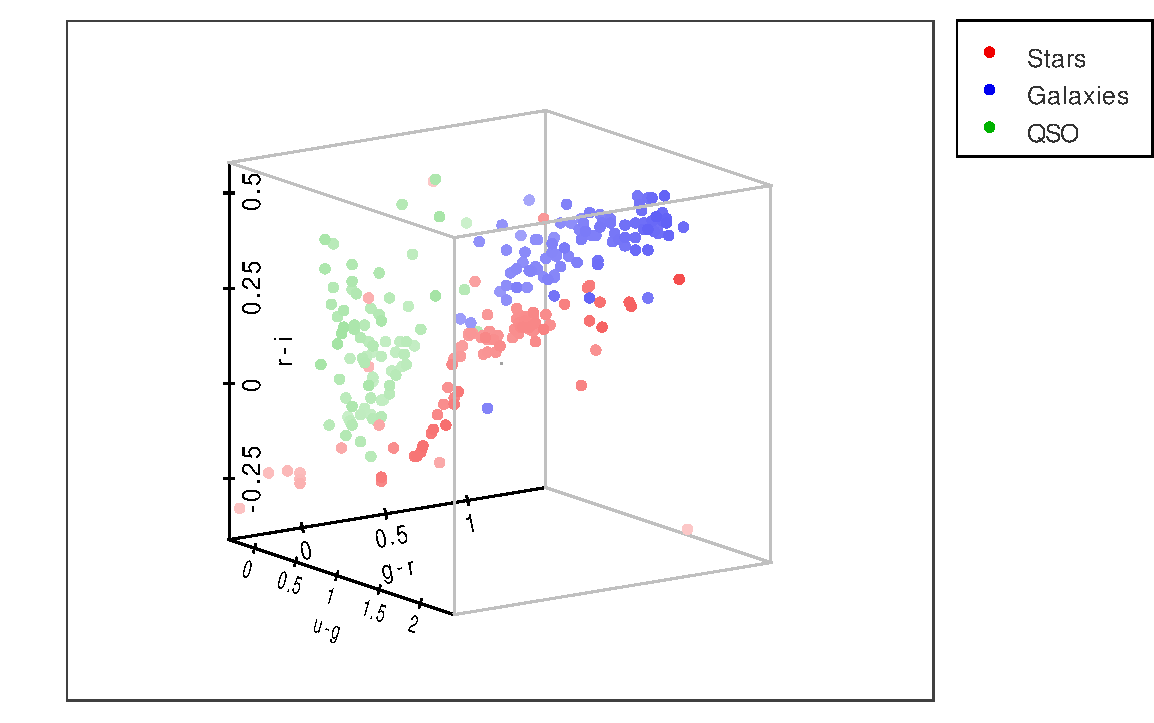
\includegraphics[scale = .7]{starsGalaxiesQSO}
        \else
        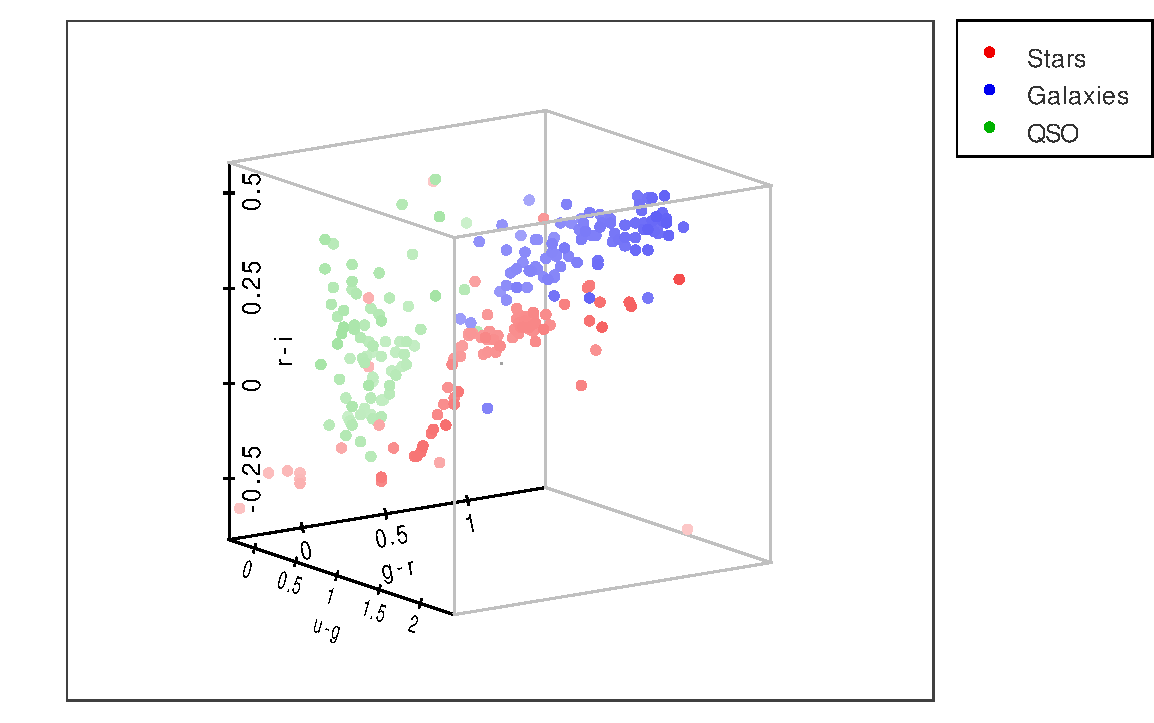
\includegraphics[bb = 92 86 545 742, height=6in]{starsGalaxiesQSO}
        \fi
        \caption{Color Diagram of the problem. It shows that individual
        objects classes occupies different region in the digram.}
        \label{FigStarsGalaxiesQSO}
 %     \end{center}
\end{figure}

\clearpage


\subsection{Support Vector Machine (SVM)}

\section{Unsupervised Methods}
\section{Existing Projects}
\subsection{Weka}
\subsection{SVM lib}
\subsection{DAME}